\chapter{Bringing pieces together: IL-10-GAG interaction insights}

In this short chapter, I assemble important insights about the IL-10-GAG system
derived during this thesis project and try to bring them into the biological
context. Some of these insights have a synergy effect, i.e.\ they support each
other and provide rather strong clues about how the IL-10-GAG system behaves in
nature on the molecular level.


\subsubsection{Experimental input: non-random, but weak interaction}

As noted in \cref{chapter:nmr}, our collaborators in Prof. Huster's NMR
laboratory at the University Leipzig could confirm binding between heparin
oligosaccharides and murine IL-10. As of the high similarity between human and
murine IL-10 (see \cref{background:il10biologyprimer}), this result is very
likely transferable between species. As published \cite{kuenze_gehrcke_2014},
the binding affinity between IL-10 and HP oligosaccharides measured in G.
Künze's NMR essays was determined to be in the micromolar range, whereas
Salek-Ardakini et al.\ found a binding affinity in the nanomolar range
\cite{salek_ardakani_2000}. Considering the differences in the investigated
systems (polymeric HP \textit{versus} oligomeric HP, human IL-10 \textit{versus}
murine IL-10) and the entirely different experimental techniques, it is no
worrying contradiction that both results differ by an order of magnitude.

The experimentally obtained binding affinity results and the computationally
obtained observation that IL-10-HP interaction has a measurable impact on the
backbone structure of HP (see \cref{chapter:nmr}) are strong clues that IL-10
and HP interact in a non-random fashion. However, various indicators point
towards a rather weak interaction, compared to e.g.\ FGF2-HP. One of these
pointers is that HP dp4's iduronic acid populates both, the ${}^1$C${}_4$ and
${}^2$S${}_\mathrm{O}$ conformations in the bound state (see
\cref{chapter:nmr}).


\subsubsection{Putative binding poses fit experimental data}

In \cref{chapter:bspred}, a putative IL-10-GAG binding region (occurring twice
as of the symmetry of the IL-10 homodimer) has been proposed, based on the
analysis of IL-10's Coulomb potential. In \cref{chapter:dmd}, it is described
how this binding region was further analyzed with DMD, and narrowed down towards
single key amino acids (being most responsible for GAG binding) and towards two
principal putative GAG binding poses, named A and B (see
\cref{fig:dmdil10:2nd_stage_principal_poses}). These poses are in the
neighborhood of R107, which has been identified as especially important for GAG
binding, and have special relations to experimentally obtained data, as will be
described in the following paragraphs.

\begin{figure}
\centering
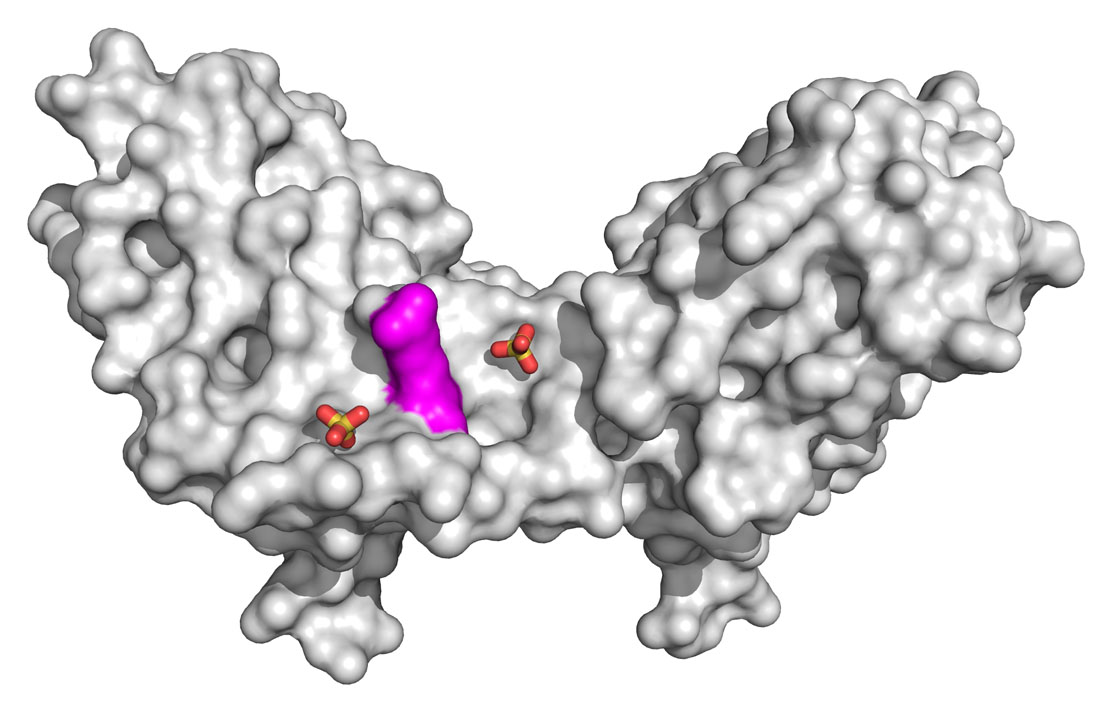
\includegraphics[width=1.0\textwidth]{gfx/together/il10sulfates_01.jpg}
\caption[]{
Structure of human IL-10 according to PDB entry 2ILK in surface representation,
including two sulfate groups contained in the crystal structure, shown in thick
stick representation. The surface of IL-10's amino acid residue R107 is colored
in magenta. During crystal growth, sulfate groups assume energetically favorable
positions, which are transferable to sulfate groups in GAGs.}
\label{fig:together:il10sulfates}
\end{figure}

In protein crystallization, salts are often used for diminishing the
electrostatic repulsion and for promoting the hydrophobic interactions among
proteins. In high-quality crystal structures, the atomic groups of salts are
spatially resolved and visible. Often, sulfates are used for facilitating the
crystal growth \cite{crystal_salts_2001}. During crystal growth, these atomic
groups end up in positions that are physically favorable for them and therefore
provide valuable input when it comes to the investigation of protein-GAG
interaction: it is valid to assume that the very same locations would also be
energetically favorable for sulfate groups contained in GAGs.

Three sulfate groups are contained in the 2ILK crystal structure of IL-10 (which
has been used throughout this thesis). Two of these sulfate groups are located
right in the neighborhood of R107, as shown in \cref{fig:together:il10sulfates}.
The location of the sulfate groups contained in the 2ILK crystal structure is a
strong experimental support of the the putative IL-10-GAG binding region
presented in \cref{chapter:bspred}. Furthermore, the imaginary line connecting
both sulfate groups aligns well with the putative GAG binding pose A that was
shown in \cref{fig:dmdil10:2nd_stage_principal_poses}. The putative GAG binding
pose B crosses the position of one of both sulfate groups.

As described in \cref{chapter:nmr}, NMR data suggests a cooperative binding mode
in which a GAG oligosaccharide bridges both symmetrically aligned putative
IL-10-GAG binding regions. In a thought experiment, extended versions of both
putative GAG binding poses, A and B, can be thought to connect both binding
regions on the front and back of the IL-10 V-shape. For binding mode B, however,
this seems to be a more probable scenario than for binding mode A.



\subsubsection{Modulation of IL-10 biology by impaired diffusion}

In literature it is often speculated that cytokine-GAG interaction for certain
systems does not directly affect the signaling cascade, but rather may be a
mechanism for cytokine concentration and diffusion control, e.g.\ for retaining
a type of cytokine close to its site of secretion in the tissue (see
\cref{background}). The question after the biological meaning of IL-10-GAG
interaction could not be answered in this project. However, the scenario in
which longer GAG chains impair the diffusion of IL-10 without affecting the
IL-10 receptor system seems to be a valid model, after the findings made in this
thesis project.

\begin{figure}
\centering
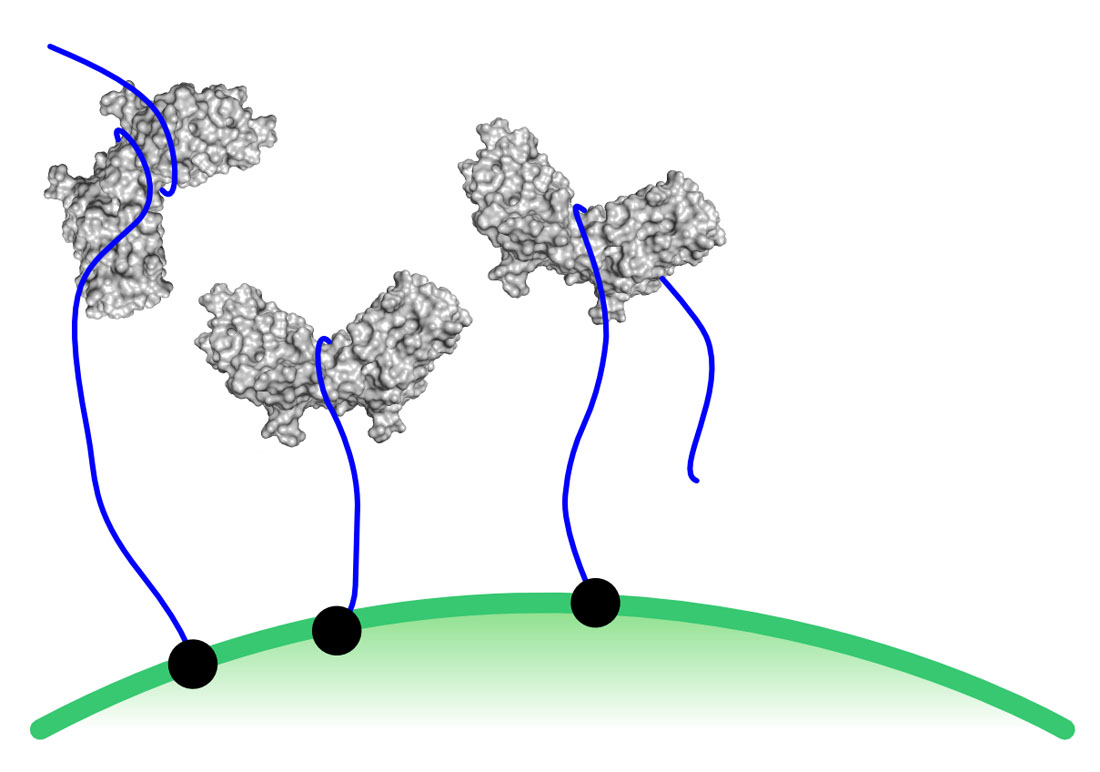
\includegraphics[width=1.0\textwidth]{gfx/together/agglomeration_small.jpg}
\caption[]{
Schematic visualization of how cell surface-attached proteoglycans (black) with
long GAG chains (blue) might impair IL-10 (gray) diffusion. The cell membrane is
here indicated in green, with the inner part of the cell being at the bottom. In
this view, the groove of IL-10's V-shape...}
\label{fig:together:il10sulfates}
\end{figure}


Show image that schematically shows how IL-10 might be caught by cell-surface-attached GAGs.



Geometrically, the putative GAG binding
pose B


which locations on the protein are
especially favorable for single sulfate groups



be concluded that both results fit.


 (two entirely different methods were used) (e.g.\ and )



NMR: IL-10-HP binding happens, measured with lower affinity than initially published by


in orientation A or B, it is more likely that a GAG can bridge both binding
regions.





\subsubsection{Modulation of IL-10 biology by interference with receptor
binding}

    - Binding region/site
    - Binding features
    - Variation of behavior among GAG types
    - Implications on biology: interference with R2, agglomeration of IL-10
    - Other hypotheses
        - Binding overlaps with R1


\hl{Note (TODO):}
Show picture of R107 specifically marked in the structure, together with
crystal sulfates, discuss possible binding poses involving these crystal
sulfates. Nee, mach das später, bei bringing it all together.

The two binding poses shown in the DMD-IL-10 chapter yeah!


\hl{Note (TODO):}
Discuss models explaining impact of IL-10-GAG interaction on IL-10 biology.



